\begin{frame}[fragile]
    \frametitle{Agglomerative Treelet Restructuring}
    \begin{lstlisting}[language=C++,basicstyle=\ttfamily,keywordstyle=\color{blue}]
for (internal node i : BVH)
    treelet = FormTreelet(i)
    clusters = treeletLeaves
    while (length(clusters) > 1)
        distances = {}
        for ((x, y) : pairs(clusters))
            d = Dissimilarity(x, y)
            distances = (d, x, y)
        (m, n) = FindMinDistance(distances)
        o = MergeClusters(m, n)
        clusters.remove(m)
        clusters.remove(n)
        clusters.add(o)
    \end{lstlisting}
\end{frame}

\begin{frame}
    \frametitle{Метрика расстояния}
    \framesubtitle{Agglomerative Treelet Restructuring}
    \begin{block}{}
        На каждой итерации пара узлов
        которые ближе друг к другу с использованием данной метрики, будут объединены.
    \end{block}

    \begin{block}{Метрика}
        Поскольку цель состоит в том, чтобы минимизировать общую стоимость SAH дерева,
        за расстояние между двумя кластерами будем считать площадь поверхности
        ограничивающей рамки, содержащей их
    \end{block}

    Это дорогая операция расстояния, поэтому есть смысл кэшировать расстояния между парами кластеров
    заранее 
\end{frame}

\begin{frame}{Треугольная матрица расстояний}
    \framesubtitle{Agglomerative Treelet Restructuring}
    \begin{columns}
        \column{0.5\textwidth}
        Удобно кэшировать расстояния между кластерами в треугольной матрице.

        Рассмотрим измениения в матрице после объединения кластеров 3 и 5
        \begin{block}{Строка и столбец по индексу массива}
            $r = 1 + \lfloor \frac{\sqrt{8i + 1}-1}{2} \rfloor$

            $c = i + \frac{r(r-1)}{2}$
        \end{block}

        \begin{itemize}
            \item 
                Красные - вычислить заново
            \item 
                Синие - скопировать
        \end{itemize}
        \column{0.5\textwidth}
        \begin{figure}
            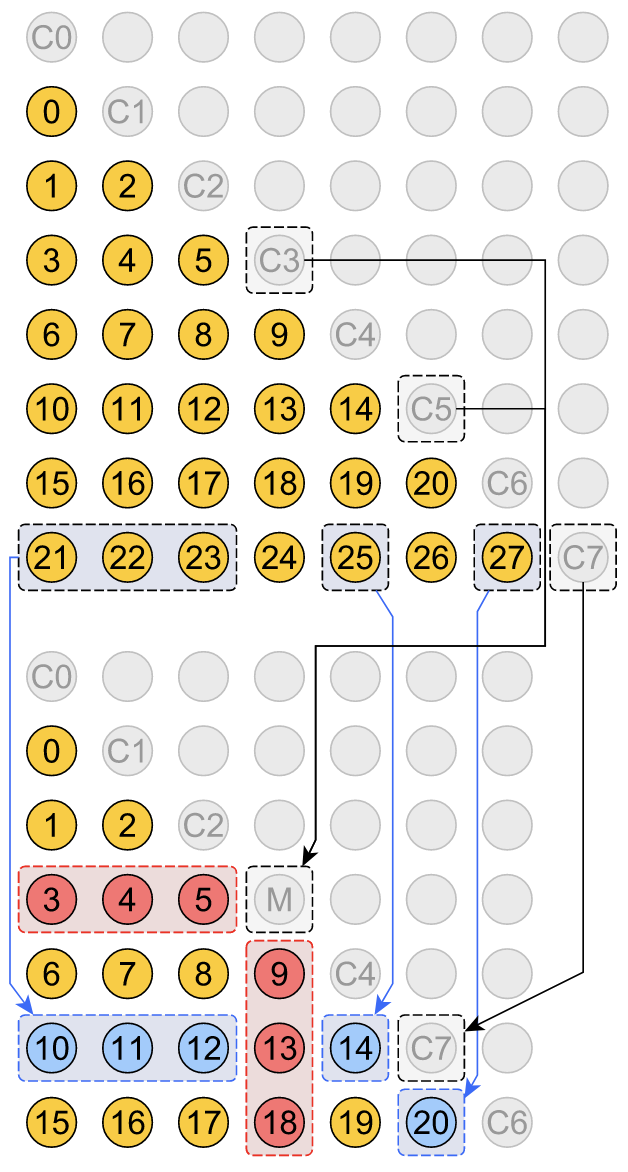
\includegraphics[height=0.75\textheight]{res/dist_matrix.png}
        \end{figure}
    \end{columns}
\end{frame}

\begin{frame}{Объединение кластеров}
    \framesubtitle{Agglomerative Treelet Restructuring}
    \begin{block}{Agglomerative clustering}
        На каждом шаге два кластера, находящиеся ближе друг к другу (по матрице расстояний) объединяются.
        Соединяем объедененные кластеры внутренним узлом (изменяя указатели)
    \end{block}

    \begin{figure}
        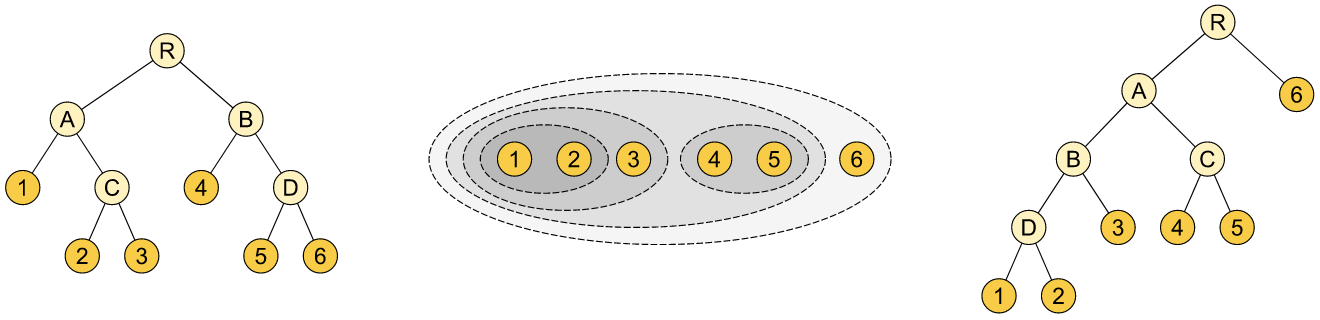
\includegraphics[keepaspectratio, width=\textwidth]{res/merge_treelets.png}
    \end{figure}

    Аллоцировать память на новые узлы не нужно.
\end{frame}

\begin{frame}[t]{SAH cost проверка}
    \framesubtitle{Agglomerative Treelet Restructuring}
    \begin{block}{}
        Все предлагаемые модификации \textbf{сохраняются в списке}, а не применяются сразу
    \end{block}
    Каждая запись списка содержит:
    \begin{itemize}
        \item 
            индекс внутреннего узла, который необходимо изменить
        \item 
            индексы двух его дочерних узлов
    \end{itemize}

    После обработки всего трилета \textit{SAH cost} новой топологии сравнивается
    с первоначальной стоимостью трилета
    \begin{block}{}
        Изменения вступят в силу только в том случае, если стоимость уменьшилась
    \end{block}

\end{frame}

\begin{frame}{Post-processing}
    \framesubtitle{Agglomerative Treelet Restructuring}

    Практика показывает, что \textit{SAH-cost} оптимизированного дерева можно еще уменьшить,
    разрушив (начать хранить примитивы напрямую) некоторые поддеревья

    \begin{block}{Стоимость \textit{разрушенного} дерева}
        \(
        c = c_t A(n) N(n)
        \)

        $n$ - subtree root

        $A()$ - площадь поверхности

        $N()$ - кол-во примитивов (треугольников) в дереве
    \end{block}
    Если полученная стоимость меньше \textit{SAH-cost} поддеревца, то принимаем решение об замене
    поддервца листом с $N(n)$ треугольников
\end{frame}

\begin{frame}{Параметры}
    \framesubtitle{Agglomerative Treelet Restructuring}
    \begin{itemize}
        \item
            размер трилета (кол-во узлов на трилет)

            Оптимальное значение: \textcolor{teal}{9}
        \item
            количество итераций (полные перестроения всей TRBVH)

            Оптимальное значение: \textcolor{teal}{2}
        \item
            $\gamma$ (сколько листьев должно быть в трилете)
    \end{itemize}

    \begin{block}{Соотношение скорость качество}
        $\gamma$ определяет может ли узел быть использован в качестве корня трилета.
        Чем больше $\gamma$ тем быстрее скорость конструкции. Уменьшение $\gamma$ приводит к улучшению качества.

    \end{block}

\end{frame}

\begin{frame}[t]{Память нужная для алгоритма}
    \framesubtitle{Agglomerative Treelet Restructuring}
    В \textit{shared memory} располагаются 3 массива:
    \begin{itemize}
        \item
            \textit{leaf indices}
        \item
            \textit{internal node indices}
        \item
            \textit{leaf surface areas}
    \end{itemize}
    \textit{Leaf surface areas} используются только при формировании трилета, так что этот массив можно использовать для других целей
    при престроении трилета.

    Когда кластеры объединяются, можно использовать последний неиспользуемый узел из \textit{internal node indices} для хранения
    информации в новом кластере.
\end{frame}

\begin{frame}[t]{Занимаемая память}
    \framesubtitle{Agglomerative Treelet Restructuring}
    \textit{52 byte of global memory} на узел:
    \begin{itemize}
        \item
            указатели на родителя и на двух дочерхних узлов
        \item
            индекс
        \item
            площадь поверхности
        \item
            \textit{AABB (32 byte)}
    \end{itemize}
    Прочие траты:
    \begin{itemize}
        \item
            атомарные счетчики
            \textit{(4 byte / node)}
        \item
            кол-во треугольников под узлом
            \textit{(4 byte / node)}
        \item
            \textit{SAH-cost} каждого узла
            \textit{(4 byte / node)}
        \item
            агломеративное расписание (необязательно)
            \textit{(256 byte / treelet size of 32)}
        \item
            матрица расстояний (при размере трилета >21)
            \textit{($\text {number of cluster combinations} * 4 \text{bytes}$ / warp)}

    \end{itemize}

\end{frame}

\begin{frame}[t]{Результаты}
    \framesubtitle{Agglomerative Treelet Restructuring}

    \begin{columns}
        \column{0.8\textwidth}

        \resizebox{\textwidth}{!}{
            \begin{tabular}{|c c c c c c|}
                \multicolumn{6}{c}{Sponza (262K)} \\
                \hline
                Method & Mrays/s & Time & SAH & Memory & Relative \\
                \hline
                LBVH & 56.17 & 7.91 ms & 114.42 & 7 MB & 69.23\% \\
                TRBVH & 81.13 & 37.86 ms & 75.75 & 50 MB & 100.00\% \\
                ATRBVH & 85.99 & 26.43 ms & 75.42 & 12 MB & 105.99\% \\
                ATRBVH* & 77.80 & 30.36 ms & 75.88 & 12 MB & 95.90\% \\
                \hline
        \end{tabular} }

        \resizebox{\textwidth}{!}{
            \begin{tabular}{|c c c c c c|}
                \multicolumn{6}{c}{Hairball (2.9M)} \\
                \hline
                Method & Mrays/s & Time & SAH & Memory & Relative \\
                \hline
                LBVH & 15.33 & 65.71 ms & 541.90 & 77 MB & 92.41\% \\
                TRBVH & 16.59 & 374.22 ms & 478.08 & 520 MB & 100.00\% \\
                ATRBVH & 16.44 & 255.24 ms & 475.72 & 121 MB & 99.10\% \\
                ATRBVH* & 16.44 & 289.69 ms & 477.46 & 121 MB & 99.10\% \\
                \hline
        \end{tabular} }

        \column{0.2\textwidth}
        \begin{figure}
            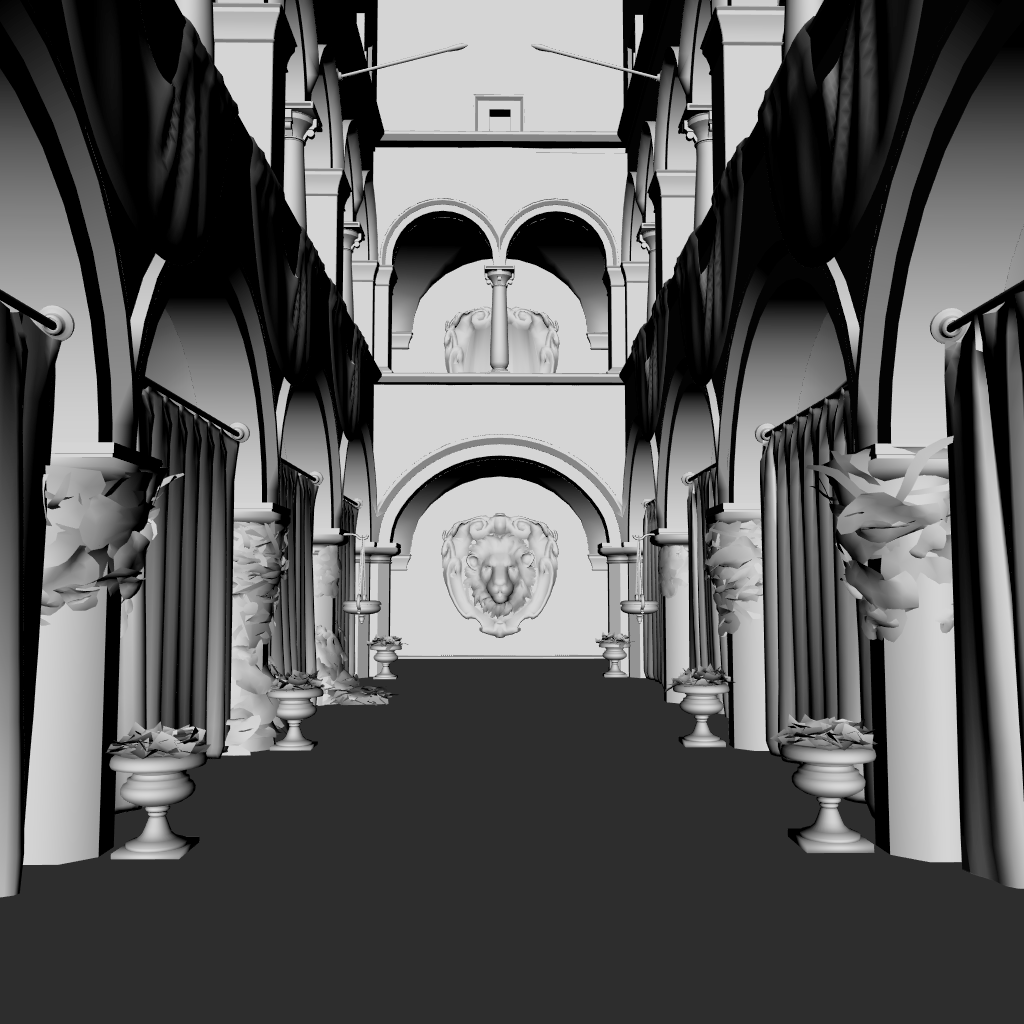
\includegraphics[keepaspectratio, width=\textwidth]{res/sponza.png}
        \end{figure}
        \begin{figure}
            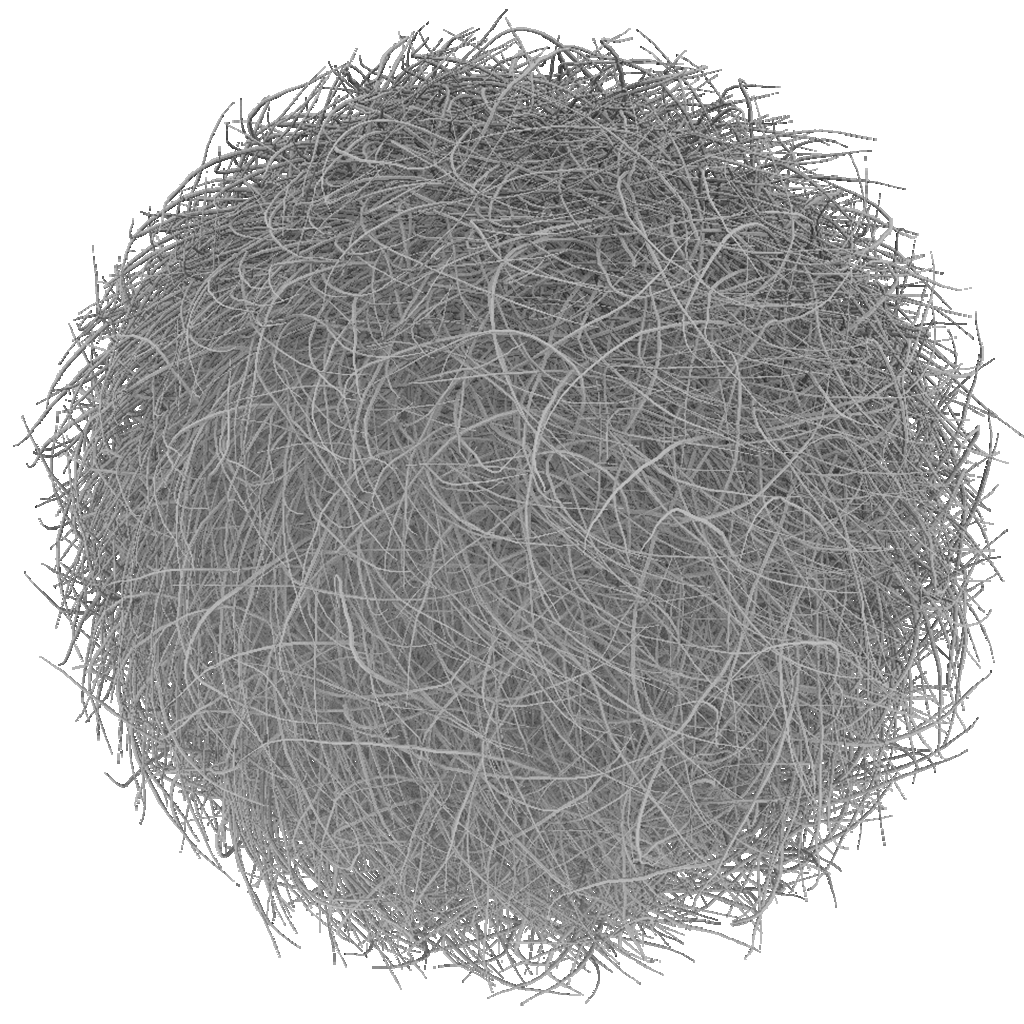
\includegraphics[keepaspectratio, width=\textwidth]{res/hairball.png}
        \end{figure}

    \end{columns}

    \begin{center}
        \resizebox{0.5\textwidth}{!}{
            \begin{tabular}{|c c c|}
                \hline
                Method & Performance (\%) & Time (\%) \\
                \hline
                LBVH & 80.8 & 20.3 \\
                TRBVH & 100 & 100 \\
                ATRBVH & 99.7 & 69.5 \\
                ATRBVH* & 99.9 & 78.4 \\
                \hline
        \end{tabular} }
    \end{center}
\end{frame}

\begin{frame}[t]
    \frametitle{Плюсы и минусы}
    \framesubtitle{Agglomerative Treelet Restructuring}
    \textbf{Достоинства}:
    \begin{itemize}
        \item
            30\% быстрее построение ATRBVH, по сравнению с базовым методом TRBVH (при схожем качестве)
        \item
            Очень параллелизируемый
        \item
            Настраиваемый и гибкий
    \end{itemize}
    \textbf{Недостатки}:
    \begin{itemize}
        \item
            Параметры не настраиваются динамически
    \end{itemize}
\end{frame}

